\section{Stand der Technik}
\label{sec:Stand der Technik}

In \ac{OSM} gibt es mehrere Arten, wie Mapper mit Flächen umgehen. So wirken einige Mapper dem Fussgängerrouting-Problem über Flächen mit zusätzlichen eingezeichneten Wegen entgegen oder die Fläche ist ganz befreit von Wegen.

In Abbildung \ref{fig:helvetiaplatz_comparison} und Abbildung \ref{fig:sechselaeutenplatz_comparison} ist ein Vergleich gängiger Routing-Engines aufgelistet, welche ein Fussgänger-Profil anbietet. In Abbildung \ref{fig:helvetiaplatz_comparison} sieht man schön, wie es bei \ac{OSM} möglich ist, dass die eingezeichneten Fusswege über denn Platz genutzt werden. Diese Route entspricht offensichtlich nicht einem natürlichen Fussgänger-Verhalten, da normalerweise der direkte Weg über den Platz gewählt wird, sofern keine Hindernisse im Weg sind. An dieser Stelle scheitert Google Maps. Der Vergleich von Google Maps und \ac{OSM} hinkt hier natürlich, da nicht beide auf den genau gleichen Datenbestand zurückgreifen. Betrachtet man in Abbildung \ref{fig:sechselaeutenplatz_comparison} hingegen den Sechseläutenplatz sieht man, dass ohne eingezeichnete Wege, alle getesteten Anbieter um den Platz herum führen.

\begin{figure}[ht]
\centering
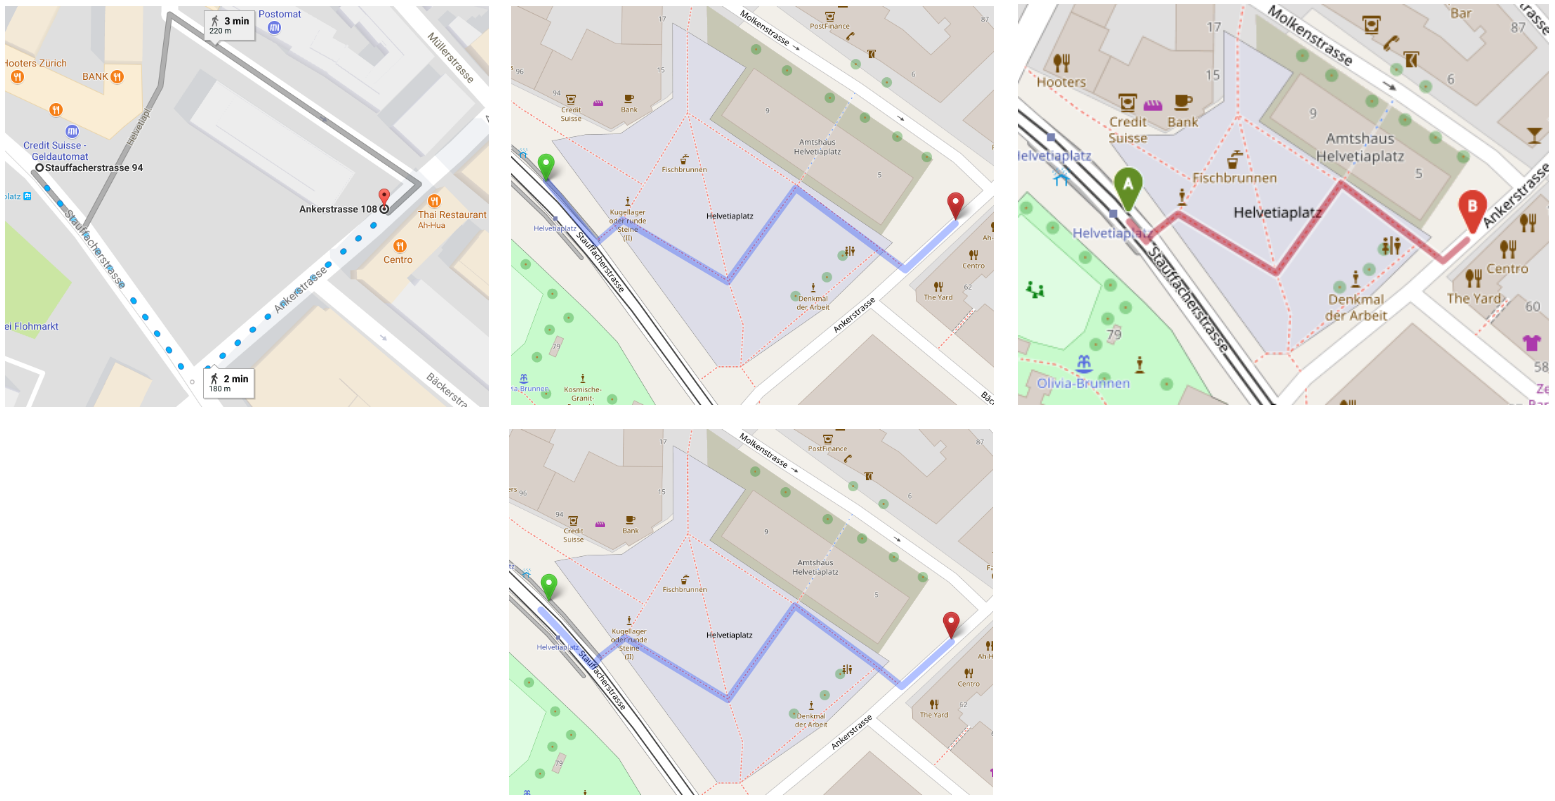
\includegraphics[width=1\linewidth]{technicalreport/img/helvetiaplatz_comparison}
\caption[Fussgänger-Routing Vergleich]{Routing-Vergleich von verschiedenen Anbietern mit Fussgänger-Profil über den Helvetiaplatz, Zürich, Schweiz; Links: Google Maps, Mitte-Oben: openstreetmap.org mit GraphHopper, Mitte-Unten: openstreetmap.org mit Mapzen, Rechts: openrouteservice.org; Screenshots aufgenommen am 13.10.2017}
\label{fig:helvetiaplatz_comparison}
\end{figure}

\begin{figure}[ht]
\centering
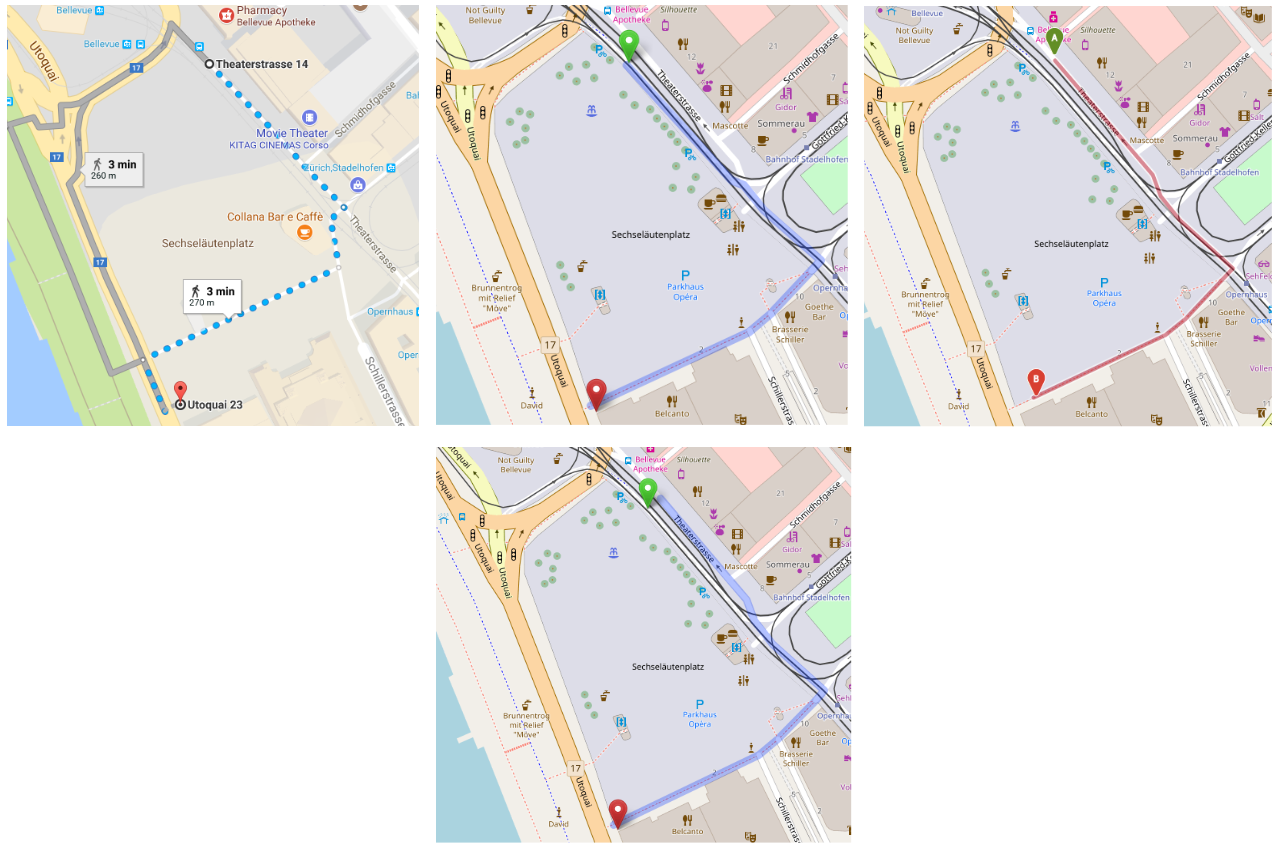
\includegraphics[width=1\linewidth]{technicalreport/img/sechselaeutenplatz_comparison}
\caption[Fussgänger-Routing Vergleich]{Routing-Vergleich von verschiedenen Anbietern mit Fussgänger-Profil über den Sechseläutenplatz, Zürich, Schweiz; Links: Google Maps, Mitte-Oben: openstreetmap.org mit GraphHopper, Mitte-Unten: openstreetmap.org mit Mapzen, Rechts: openrouteservice.org; Screenshots aufgenommen am 13.10.2017}
\label{fig:sechselaeutenplatz_comparison}
\end{figure}


Abschliessend kann man sagen, dass alle getesteten Routing-Engines mit den Fussgänger-Profilen mit Stand 13.10.2017 scheitern, wenn keine Wege über die Fläche eingezeichnet sind und so die Dauer und Streckenlänge verfälscht wird.

\subsection{Bestehende Lösungsansätze}
\label{sub:Bestehende Lösungsansätze}


\subsubsection{Routing über offene Flächen}
\label{solution:Routing über offene Flächen}

Diese Arbeit nimmt Bezug auf zwei Lösungsansätze \cite{graser_visibility_graph}, \cite{dzafic_spider_web_graph}, welche sich aus verschiedenen Motivationsgründen mit dem Problem \ref{problem:Routing über offene Flächen} befassen. Diese werden in den folgenden Unterkapitel erläutert. Mit Pseudocode wird der Ansatz verdeutlicht. Beide Varianten werden in QGIS getestet. 

Zum Schluss wird ein Variantenvergleich durchgeführt und ein Fazit gezogen. Ziel ist es, einen Flächen-Routing-Algorithmus zu finden, welche für die Vorverabeitung der Flächen verwendet werden kann.  

\paragraph{Visibility Graph}~\\

TODO

\paragraph{Spider-Web Graph}~\\


Die Arbeit \cite{dzafic_spider_web_graph} befasst sich mit dem Flächenrouting für Nutzern von Elektrorollstühlen, indem ein Spinnennetz (siehe Abbildung \ref{fig:spiderweb}) über das Polygon gelegt wird. Dies hat den Vorteil, dass auf dem Polygon, sprich der Fläche zusätzliche Linien und Kanten vorhanden sind, wobei statische Hindernisse berücksichtigt werden, welche für das Routing verwendet werden können. Diese Idee und das Grundprinzip wurde im folgenden übernommen.

\begin{figure}[ht]
\centering
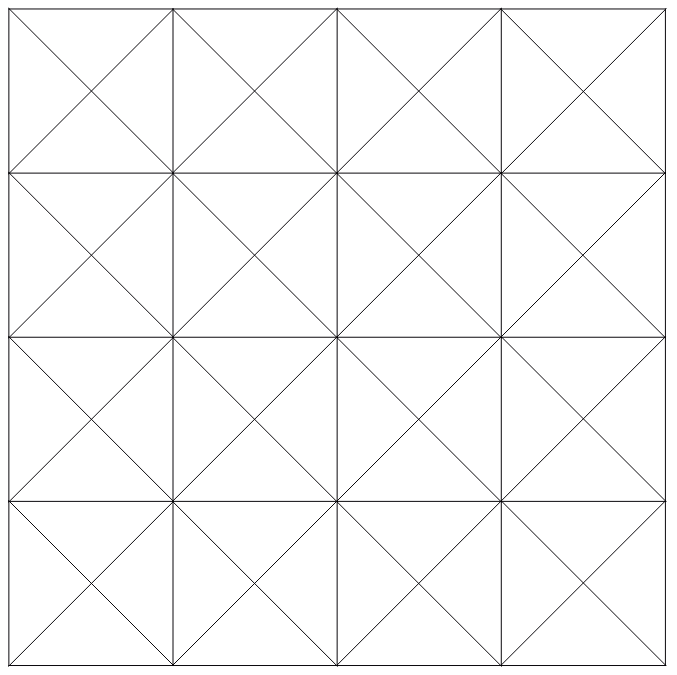
\includegraphics[width=0.5\linewidth]{technicalreport/img/spiderweb}
\caption[Spinnennetz]{Spinnennetz}
\label{fig:spiderweb}
\end{figure}

Zur Verdeutlichung der Idee ist der Pseudocode \ref{Spiderweb Pseudocode} in zu betrachten.

\begin{listing}[ht]
    \inputminted{python}{technicalreport/listing/spiderweb_pseudocode.py}
    \caption{Spiderweb Pseudocode}
    \label{Spiderweb Pseudocode}
\end{listing}

Vor dem Zeichnen des Spinnennetz ist es möglich, den Abstand zwischen Spalten und den Zeilen (Spacing) zu definieren. Dies hat hohe Auswirkung auf die gezeichneten Pfade über die Fläche, da mit einem kleineren Spacing eine "Glättung" der Pfade möglich ist. Die gezeichneten Pfade widerspiegeln so eher das Verhalten eines Fussgängers. Ein Abstrich des kleiner Spacings ist sofort ersichtlich, wenn man das Spinnennetz in der Abbildung \ref{fig:spiderweb} betrachtet. Man kann annehmen, dass dieses Spinnennetz über eine Fläche von 4*4 cm mit einem Spacing von einem 1 cm gezeichnet wird. Verkleinert man nun das Spacing auf 0.5cm steigt die Anzahl der zu zeichnenden Linien von ... auf .... Somit haben wir einen Speicherbedarf von O(???). Da nun in diesem Fall x Mal mehr Lininen verfügbar sind, steigen auch die Anzahl möglicher Pfade über die Fläche ... an, was Auswirkung auf die Generierung des Shortest Paths hat. 

Es wurde ebenfalls geprüft, ob die Rotation des Spinnennetz auf die Gegebenheit der Fläche einen Auswirkung auf die Shortest Path-Generierung hat. Bei einem Test, welcher in Abbildung \ref{fig:rotation_comparison} ersichtlich ist, wurden keine entscheidenden Vorteile gefunden, warum sich der zusätzliche Aufwand rechtfertigen würde. Das Spinnennetz wurde um 45 und um 90 Grad gedreht. Die berechneten kürzesten Pfade sind fast identisch.

\begin{figure}[th]
\centering
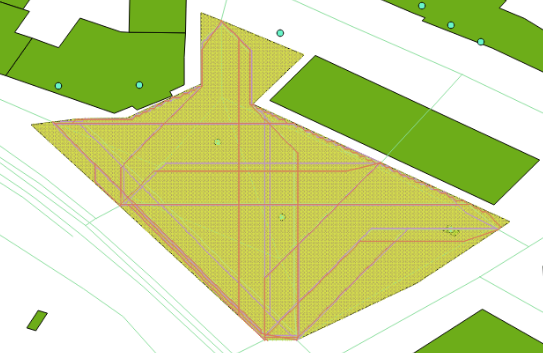
\includegraphics[width=0.7\linewidth]{technicalreport/img/rotation_comparison}
\caption[Rotation Comparison]{Rotation des Spiderwebs um 45 und 90 Grad im Vergleich mit keiner Rotation}
\label{fig:rotation_comparison}
\end{figure}


\paragraph{Einschränkungen}~\\

TODO
% TODO mögliche Einschränkungen, welche die Varianten in ihrer Anwendung betreffen

\paragraph{Vergleich}~\\

TODO

% TODO Gegenüberstellung der Varianten, welche ist in welcher Situaiton sinnvoll

\paragraph{Fazit}~\\

TODO

% TODO Welche Variante wird verwendet

\subsection{Kurzbeschreibung und Charakterisierung}
\label{sub:Kurzbeschreibung und Charakterisierung}
TODO

\subsection{Defizite}
\label{sub:Defizite}
% Hinweise auf Weiterentwicklungs-, bzw. Verbesserungspotential
TODO
% hier Probleme, welche im Visiblity Graph Paper erwähnt sind aufgreifen.
